\documentclass[conference]{IEEEtran}
\IEEEoverridecommandlockouts
\usepackage{amsmath,amssymb,amsthm}
\usepackage{graphicx}
\usepackage{booktabs}
\usepackage{xcolor}
\usepackage{url}
\usepackage[hidelinks]{hyperref}
\usepackage{cite}

% Inline to-do marker (no margin notes in two-column IEEEtran).
\newcommand{\todo}[1]{\textcolor{red}{[\textsc{todo}: #1]}}
\newtheorem{proposition}{Proposition}
\newtheorem{corollary}{Corollary}

\begin{document}

\title{\todo{title}}

\author{\IEEEauthorblockN{Shashwat \todo{full name}}
\IEEEauthorblockA{BITS Pilani \todo{department, campus}\\
\todo{email}}}

\maketitle

% ---------------------------------------------------------------- results-dependent: written after the analysis
\begin{abstract}
\todo{abstract: written after the blind analysis}
\end{abstract}

\section{Introduction}\label{sec:intro}
\todo{introduction and contribution list: written after the blind analysis}

% ---------------------------------------------------------------- results-independent sections
\section{Related Work}\label{sec:related}

\textbf{Graph-based retrieval memory.}
HippoRAG~\cite{gutierrez2024hipporag} builds a schemaless knowledge graph from a corpus with an LLM and retrieves
passages by Personalized PageRank (PPR) seeded from query entities, modelled on the hippocampal indexing theory of
memory. HippoRAG~2~\cite{gutierrez2025hipporag2} adds passage nodes to the graph and an LLM recognition-memory filter
over candidate facts, and frames the system as non-parametric continual learning: new knowledge is absorbed by
indexing, without changing model weights. GraphRAG~\cite{edge2024graphrag} builds an entity graph and pre-generated
community summaries for corpus-level sensemaking queries. LightRAG~\cite{guo2024lightrag} combines graph-based
indexing with dual-level (entity and theme) retrieval and an incremental update algorithm. RAPTOR~\cite{sarthi2024raptor}
recursively clusters and summarises chunks into a tree and retrieves across its levels. None of these evaluates what
happens when newly indexed text contradicts what the index already holds; that is the question studied here.

\textbf{Poisoning retrieval-augmented generation.}
PoisonedRAG~\cite{zou2025poisonedrag} shows that a few injected texts per target question can steer a RAG system to an
attacker-chosen answer. For graph-based RAG, GraphRAG under Fire~\cite{liang2025graphragfire} reports that graph
indexing resists simple poisoning but opens new attack surfaces, and exploits shared relations to poison many queries at
once. KEPo~\cite{chen2026kepo} argues that text-level attacks fail against GraphRAG because the knowledge-graph
abstraction reorganises injected text, and instead forges a chain of knowledge evolution ending in the poisoned fact.
On the defence side, HoG-GRAG~\cite{noughabi2026defense} decomposes multi-hop questions and checks each hop for
poisoning-induced inconsistencies, and PURPOSE~\cite{wang2026purpose} attacks the post-retrieval conflict-resolution
step itself. To a retriever, an injected correction and an injected poison are the same operation: new passages that
contradict stored ones. This work measures the benign side of that operation on HippoRAG~2, with the same
injection mechanics but no adversarial optimisation of the injected text.

\textbf{Memory systems with explicit updates.}
Zep~\cite{rasmussen2025zep} maintains a bi-temporal knowledge graph for agent memory, recording when facts held and when
they were ingested, so that superseded facts can be invalidated. Mem0~\cite{chhikara2025mem0} extracts salient facts from
conversations and applies explicit update operations, with a graph variant. Contradiction-aware updating is therefore
not new; the contradiction-aware seeding tested here is an intervention used to locate where HippoRAG~2 loses a
correction, evaluated under oracle detection (Section~\ref{sec:method}).

\textbf{Knowledge conflicts.}
Longpre et al.~\cite{longpre2021entity} substitute answer entities in retrieved passages and find that reader models
often fall back on memorised answers. ClashEval~\cite{wu2024clasheval} finds that LLMs adopt incorrect retrieved content
over a correct prior in a large share of cases, and that adoption depends on the model's confidence in its prior. Both
study the reader given a fixed context. Here the question is upstream: whether the retriever surfaces the corrected
passage at all. The long-context arm (Section~\ref{sec:method}) connects the two by giving the reader every passage.

\section{Background: HippoRAG 2 Retrieval as Stages A--E}\label{sec:background}

All values below are read from the released code (\texttt{src/hipporag}, version 2.0.0a5, tag \texttt{upstream-base},
commit \texttt{d5c8329}); Table~\ref{tab:defaults} lists the defaults that matter for retrieval.

\textbf{Index.} An OpenIE pass extracts $(s, r, o)$ triples from every passage. Normalised subjects and objects become
phrase nodes and every passage becomes a passage node. A passage is linked to each phrase in its triples by an edge of
weight~1. Each triple adds a fact edge between its subject and object whose weight is the number of passages asserting
it (one source count per passage), so re-asserting a fact in more passages strengthens its edge. Synonym edges connect
phrase pairs with embedding cosine $\ge 0.8$. The graph is undirected; the relation label is not stored on the edge.
A second \texttt{index()} call adds only new passages, facts and phrases, and computes synonym edges only for the new
phrases.

\textbf{Retrieval} runs five stages per query (Fig.~\ref{fig:pipeline}):
\begin{itemize}
\item[A] \emph{Fact candidates.} All facts are scored by the dot product between the query embedding and each fact's
embedding, min--max normalised; the top \texttt{linking\_top\_k}$\,=5$ become candidates.
\item[B] \emph{Recognition filter.} One LLM call with a few-shot DSPy prompt keeps the candidates it judges relevant
(at most 5). If none survive, the query falls back to dense passage retrieval and stages C--D are skipped.
\item[C] \emph{Seeds.} Each subject and object of a kept fact receives the fact's score divided by the number of
passages containing that phrase, averaged over its occurrences; only the top 5 phrases keep their weight. Every passage
receives its min--max normalised dense score times \texttt{passage\_node\_weight}$\,=0.05$. Together these form the
reset vector.
\item[D] \emph{Personalized PageRank} over the weighted undirected graph (python-igraph, PRPACK), damping $0.5$.
\item[E] \emph{Top 5.} Passages are ranked by PPR score; the reader sees the top \texttt{qa\_top\_k}$\,=5$.
\end{itemize}

\begin{table}[t]
\centering
\caption{HippoRAG 2 retrieval defaults (code, \texttt{utils/config\_utils.py}), unchanged in every run here.}
\label{tab:defaults}
\resizebox{\columnwidth}{!}{%
\begin{tabular}{lll}
\toprule
Parameter & Value & Role \\
\midrule
\texttt{linking\_top\_k} & 5 & facts to the filter; facts and phrases kept \\
\texttt{passage\_node\_weight} & 0.05 & weight of dense scores in the reset \\
\texttt{damping} & 0.5 & PPR damping \\
\texttt{retrieval\_top\_k} & 200 & passages returned \\
\texttt{qa\_top\_k} & 5 & passages given to the reader \\
\texttt{synonymy\_edge\_sim\_threshold} & 0.8 & synonym-edge cosine threshold \\
\texttt{synonymy\_edge\_topk} & 2047 & neighbours searched (at most 100 kept) \\
\texttt{is\_directed\_graph} & false & undirected graph and PPR \\
\texttt{temperature} & 0 & OpenIE, filter and reader \\
\bottomrule
\end{tabular}}
\end{table}

\begin{figure*}[t]
\centering
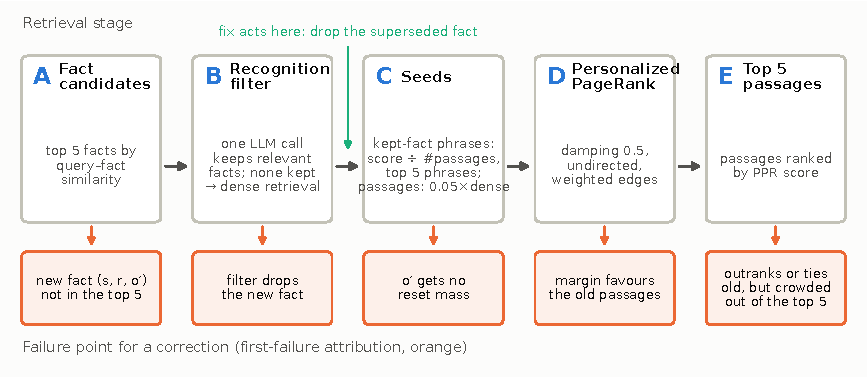
\includegraphics[width=0.9\textwidth]{figs/pipeline.pdf}
\caption{HippoRAG 2 retrieval as stages A--E (top) and the point at which a correction can be lost at each stage
(bottom), which defines the first-failure attribution of Section~\ref{sec:method}. The contradiction-aware fix acts
between B and C.}
\label{fig:pipeline}
\end{figure*}

\section{Theory: A Toy Graph}\label{sec:theory}

The protocol's prediction is written before any run (Section~\ref{sec:method}). To make it concrete, consider the
smallest graph that contains a correction (Fig.~\ref{fig:toy}). A shared subject $e$ has an old object $D$, asserted
by $n$ passages that each contain $(e, D)$, and a new object $M$, asserted by $k$ passages that each contain $(e, M)$.
Passage edges have weight 1. \emph{Graph A} has passage edges only. \emph{Graph B} adds HippoRAG's count-weighted
relation edges: $e$--$D$ with weight $n$ and $e$--$M$ with weight $k$. The reset vector puts $r_e$ on $e$, $r_D$ on $D$,
$r_M$ on $M$, $r_o$ on each old passage and $r_m$ on each new passage. PPR uses the igraph convention: damping $d$ is the
probability of following an edge, so $\pi = (1-d)\,r + d\,W^\top \pi$ with $W$ the row-normalised weighted adjacency
matrix. Write $x$ for the score of one old passage and $y$ for one new passage.

\begin{proposition}[Shared-subject seed]\label{prop:shared}
With all reset mass on the shared subject ($r_e = 1$),
\begin{align}
\text{Graph A:}\quad x = y &= \frac{d}{(1+d)(n+k)},\\
\text{Graph B:}\quad x = y &= \frac{d}{(2+d)(n+k)}.
\end{align}
\end{proposition}
Seeding only the shared subject therefore never separates old from new passages, whatever $n$ and $k$ are: redundancy
lowers every passage's score equally.

\begin{proposition}[Margin in Graph B]\label{prop:margin}
For a general reset vector,
\begin{equation}
\Delta = x - y = \frac{2(1-d)}{4-d^2}\Big[d\Big(\frac{r_D}{n} - \frac{r_M}{k}\Big) + 2\,(r_o - r_m)\Big],
\label{eq:margin}
\end{equation}
and the coefficient of $r_e$ is $0$.
\end{proposition}
The old passages win ($\Delta > 0$) only through object-specific phrase seeds ($r_D$ versus $r_M$, divided by the number
of passages on each side) and through per-passage seeds ($r_o$ versus $r_m$). Inside the bracket the passage-seed term
has weight $2$ and the phrase term weight $d$, i.e.\ $4\times$ at HippoRAG's $d = 0.5$. For reference, the same derivation for
Graph A gives $\Delta_A = \frac{2(1-d)}{2-d^2}\big[d(r_D/n - r_M/k) + (r_o - r_m)\big]$, again independent of $r_e$.

\begin{corollary}[HippoRAG's seed rule]\label{cor:seed}
HippoRAG divides a phrase's fact score by the number of passages containing the phrase (stage C). If $D$ and $M$ receive
the same fact score $\sigma$ and no passage seeds differ, then $r_D = \sigma/n$, $r_M = \sigma/k$ and
\begin{equation}
\Delta = \frac{2(1-d)}{4-d^2}\; d\,\sigma\Big(\frac{1}{n^2} - \frac{1}{k^2}\Big).
\end{equation}
The side with fewer passages gains per passage: with equal fact scores, a single correction ($k = 1$) against
redundant old support ($n > 1$) has the larger per-passage seed.
\end{corollary}

These are toy-graph results. The real index adds synonym edges, many unrelated facts and passages, min--max
normalisation, top-5 phrase truncation and dense passage seeds for every passage, so the closed forms locate mechanisms
rather than predict magnitudes. Three mechanisms follow: a correction can lose because its object is never seeded
(\emph{seed exclusion}; stages A--C), because old passages crowd the top 5 (\emph{top-5 contamination}; stage E), or
because the seeds that do differ favour the old side (\emph{graph asymmetry}; the bracket in~\eqref{eq:margin}).
All four statements were re-derived symbolically with sympy and checked against igraph's PRPACK solver on the full
(unreduced) toy graph for $n, k \in \{1,2,3,5\}$, $d \in \{0.3, 0.5, 0.85\}$ and 480 random reset vectors (maximum
absolute deviation $2.2\times10^{-16}$; \texttt{experiments/theory/verify\_margin.py}).

\begin{figure}[t]
\centering
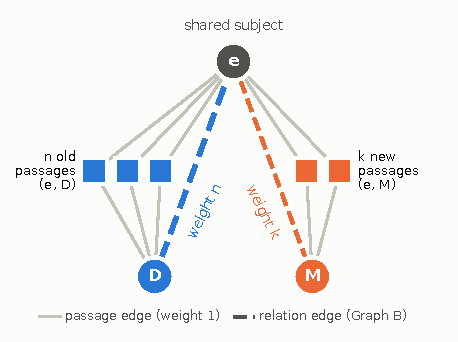
\includegraphics[width=0.82\columnwidth]{figs/toy_graph.pdf}
\caption{The toy graph ($n = 3$, $k = 2$ drawn). Graph A has the passage edges only; Graph B adds the count-weighted
relation edges $e$--$D$ (weight $n$) and $e$--$M$ (weight $k$).}
\label{fig:toy}
\end{figure}

\section{Method and Setup}\label{sec:method}

\textbf{Data and models.} MuSiQue~\cite{trivedi2022musique} as released with HippoRAG~2: 1,000 questions over a corpus
of 11,656 passages. Every LLM role uses gpt-4o-mini (OpenIE, the recognition filter, the reader, and the target
generator, checker and probe below) and every embedding uses text-embedding-3-small, instead of the paper's
Llama-3.3-70B and NV-Embed-v2. Calls go through an OpenAI-compatible gateway at temperature 0. The OpenIE triples are
the authors' released gpt-4o-mini extractions, so indexing the corpus makes no OpenIE calls. Reproduction and
extension both run the unmodified \texttt{src/} (tag \texttt{upstream-base}); extension code subclasses HippoRAG and
never edits it.

\subsection{Counterfactual targets}\label{sec:targets}
A target is a question whose answer is the object $o$ of exactly one cached triple $(s, r, o)$ across its supporting
passages, with $s$ and $o$ verbatim in that passage, $o$ not in its title and not inside another entity of its triples.
Relations where the subject already has two or more distinct objects in the corpus are dropped (a swap on a
multi-valued relation adds a value rather than correcting one). The corrected passage replaces $o$ by a counterfactual
$o'$ in the text and in the passage's cached triples. Choosing $o'$ took five iterations, each changed for a stated
reason:
\begin{itemize}
\item[v1] $o'$ drawn at random from objects seen with the same relation elsewhere. Many swaps were implausible
(``Brooklyn College is part of the FA Cup'').
\item[v2] gpt-4o-mini picks $o'$ from the 8 same-relation objects nearest to $o$ in embedding space, or answers
``none'', and states whether the relation is single-valued. The single-valued question was ineffective (284 yes, 1
no); the corpus filter above does that work. Most picks were still implausible.
\item[v3] A 1--5 plausibility rating kept only 32 of 158 picks, from just 21 distinct gold passages: several questions
share a gold passage and therefore an identical swap. From here on the unit is the distinct gold passage, with one
question per passage chosen by a seeded draw, and $n$ counts distinct swaps.
\item[v4] gpt-4o-mini generates three replacements of the same fine-grained type that are plausible in the exact
sentence and false; the first passing the offline checks (not $o$, not an answer alias, no substring either way, not in
the question's own paragraphs, the same surface shape, no doubled token at the swap boundary) is used. The 1--5 rater
kept 58 of 132, but it scored truth rather than believability: it rejected swaps whose true value it knew, which would
bias the sample towards facts the model does not know.
\item[v5] The rater is replaced by three yes/no checks that explicitly ignore the true value: same fine-grained type,
grammatical and coherent, and no impossibility a reader who does not know the fact would spot. A separate closed-book
probe, given the gold passage's title, subject and relation, records whether the model knows $o$
(\emph{model\_knows\_o}); it is a covariate, not a filter.
\end{itemize}
The v5 funnel: 139 distinct gold passages pass the anchor and single-valued rules; 132 have a generated $o'$ passing the
offline checks; 125 pass all three checks; a seeded cap keeps 120. Of these, the probe answers $o$ for 48 and not for
72; $o'$ is absent from the corpus for 62, occurs in 1--9 passages for 41 and in 10 or more for 17 (passages whose
triples contain the entity). Every swap is then reviewed by hand; the analysis uses only the kept swaps
(\todo{final count after hand review}). Analysis splits by a covariate only where every bin has at least 15 swaps.

\subsection{Injection, grid and systems}\label{sec:grid}
\textbf{Swap and variants.} The swap is deterministic: $o \to o'$ at word boundaries in the passage body, and in triple
fields that equal $o$ exactly. Extra copies of the old passage and copies of the corrected passage differ only in a
title tag (four hex characters of an MD5 of target, role and copy index), so each copy is a distinct chunk while
carrying identical triples. Identical triples collapse to one fact whose edge weight grows by one per passage; a copy's
text does not depend on the grid cell. The injected triples are written into the OpenIE cache under the same
provenance stamp, so indexing makes no OpenIE call.

\textbf{Grid.} Old support $n \in \{1, 3\}$ (the original gold passage plus $n-1$ copies) crosses corrections
$k \in \{0, 1, 2, 3, 5\}$. All targets are injected into one index per cell, cloned from the base index with APFS
copy-on-write and indexed incrementally. Targets that share a normalised entity or a gold passage are placed in
different collision-free groups by greedy colouring, and each group gets its own index per cell (two groups, of 115
and 5 swaps before hand review). Every injected passage, new fact, new entity and question is embedded once and the
vectors are reused in every cell, because repeated embedding calls are not bit-identical.

\textbf{Systems.} Three systems are compared on the same index and the same frozen vectors: \emph{dense} retrieval,
\emph{HippoRAG~2} as released, and \emph{HippoRAG~2 + fix}. The fix runs after the recognition filter: if two kept facts
share subject and relation but differ in object, it keeps the more recently inserted one (most recent insertion among
the passages asserting each fact; the base corpus is oldest) and drops the other. Detection is exact string match on the
normalised $(s, r)$. Because the corrected triple shares $s$ and $r$ with the old one by construction, this is an
\emph{oracle} detector: the fix measures resolution under perfect detection, and detection quality is out of scope.
Facts other than the target's that the fix drops (possible for multi-valued relations re-asserted by a copy) are
counted and reported as collateral drops.

\subsection{Metrics and attribution}\label{sec:metrics}
For each target and cell: \emph{correction@5}, whether any corrected passage is in the top 5 ($k \ge 1$);
\emph{contamination@5}, the number of old passages in the top 5; and whether the best corrected passage
\emph{outranks}, \emph{near-ties} or \emph{loses} to the best old passage. The third uses a relative tolerance $\tau$
(near-tie when $|s_\text{new} - s_\text{old}| \le \tau \max(|s_\text{new}|, |s_\text{old}|)$) applied at analysis time
to the raw scores (PPR for HippoRAG, cosine for dense), reported at $\tau \in \{0, 0.5, 1, 2\}\%$. Differences between
systems are reported per $(n, k)$ with paired bootstrap 95\% intervals over targets (10,000 resamples, seed 0).

Every HippoRAG failure ($k \ge 1$, correction not in the top 5) is attributed to the first stage that fails
(Fig.~\ref{fig:pipeline}): \textbf{A} the new fact $(s, r, o')$ is not among the five candidates; \textbf{B} the filter
does not keep it (after the fix, for the fix arm); \textbf{C} $o'$ receives no reset mass (including the dense
fallback); \textbf{D} the PPR margin favours the old passage beyond $\tau$; otherwise the correction is outside the top 5
although it ties (\textbf{E}$_\text{tie}$) or outranks (\textbf{E}$_\text{crowd}$) the old passage. The order and the
stage predicates are configurable. The per-query trace is computed by re-running upstream \texttt{retrieve()}'s
per-query loop with logging overrides; it is checked to reproduce upstream's ranking and scores exactly.

\textbf{Long-context reader.} At the four corners $(n, k) \in \{(1,1), (1,5), (3,1), (3,5)\}$ the reader receives the
question's own MuSiQue paragraphs plus every injected copy for that target, in a seeded random order, with HippoRAG's
reader prompt. Its answer is labelled $o'$, $o$, both or neither by normalised phrase containment. This separates
retriever failures from reader failures.

\subsection{Blind protocol}\label{sec:blind}
The full grid, the fix arm and the long-context corners were run before the hand review of the swaps and before the
prediction was written, and no result was inspected. Each (cell, group) run had to pass structural gates or abort:
zero OpenIE calls; zero embedding calls (the embedding client was patched to raise); every injected passage present in
the graph and the stores; an identical filter prompt in the fix and no-fix arms for every question; and, for five
random questions, a traced ranking identical to upstream \texttt{retrieve()}. All 20 (cell, group) runs passed. The
SHA-256 of every result file was then recorded with the timestamp 2026-11-09 04:16:16 IST (commit \texttt{c68a13e}),
before any analysis. \todo{commit hash of the prediction, written before unsealing}.

\section{Reproduction Results}\label{sec:repro}

The target is the gap between HippoRAG~2 and dense retrieval with the same embedder, not the paper's absolute numbers.
Both systems index all 11,656 passages; evaluation uses the first $N$ questions of the released 1,000-question sample.
Dense retrieval ranks with HippoRAG's own passage vectors (copied, SHA-256 identical), so the comparison isolates the
graph. All runs use the unmodified code at \texttt{upstream-base}.

\begin{table}[t]
\centering
\caption{MuSiQue reproduction (gpt-4o-mini, text-embedding-3-small). Paper: Llama-3.3-70B, NV-Embed-v2, $N = 1{,}000$.}
\label{tab:repro}
\begin{tabular}{llrrr}
\toprule
$N$ & System & Recall@5 & F1 & EM \\
\midrule
100 & HippoRAG 2 & 59.75 & 48.48 & 38.0 \\
    & Dense      & 55.25 & 40.30 & 31.0 \\
500 & HippoRAG 2 & 62.00 & 44.93 & 30.8 \\
    & Dense      & 56.10 & 40.27 & 27.6 \\
\midrule
1,000 (paper) & HippoRAG 2 & 74.7 & 48.6 & -- \\
              & Dense      & 69.7 & 45.7 & -- \\
\bottomrule
\end{tabular}
\end{table}

At $N = 500$ the gap is $+5.90$ Recall@5 points (paired bootstrap 95\% CI $[+3.73, +8.00]$) and $+4.66$ F1 points
($[+1.52, +7.69]$); EM $+3.20$ ($[+0.00, +6.40]$). The paper's gaps ($+5.0$ and $+2.9$) fall inside both intervals,
and both reproduced gaps exclude zero (Fig.~\ref{fig:repro}). Per question, HippoRAG~2 is better on Recall@5 for 113
questions, dense for 52, and they tie on 335; for F1 the split is 90 / 61 / 349. At $N = 100$ the intervals (computed on
the first 100 questions of the $N = 500$ runs, which reproduce the $N = 100$ run's Recall@5 and EM exactly) are too
wide to read the F1 gap: Recall@5 $+4.50$ $[-0.50, +9.67]$, F1 $+7.84$ $[+0.49, +15.51]$. \todo{compare the F1 with a
gpt-4o-mini reader against the paper's Appendix C, Table 8.}

Reruns are not exactly reproducible at the answer level even with the LLM cache: query embeddings are fetched again and
are not bit-identical, which reordered the top 5 for 2 of 400 questions and changed their reader prompts. The extension
avoids this by freezing every vector (Section~\ref{sec:grid}).

\begin{figure}[t]
\centering
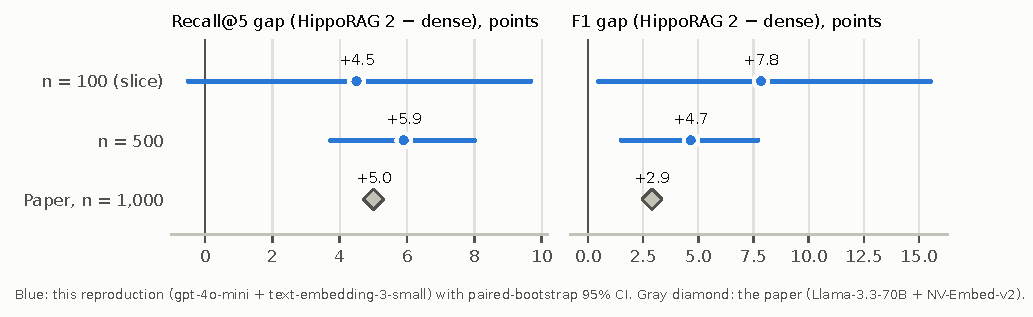
\includegraphics[width=\columnwidth]{figs/repro_gap.pdf}
\caption{HippoRAG 2 minus dense, in points, with paired-bootstrap 95\% intervals; the paper's gap for reference.}
\label{fig:repro}
\end{figure}

\section{Update-Resistance Results}\label{sec:extension}
% Stubs only. Fill by running, after the prediction is committed:
%   .venv/bin/python experiments/extension/analysis.py --results results/extension/grid_v5_20261109 \
%       --targets experiments/extension/data/targets_v5.jsonl \
%       --final experiments/extension/data/targets_final.jsonl \
%       --out <analysis_dir> --tex_dir paper/tables
% and copying <analysis_dir>/*.png into paper/figs/results/.

\todo{results text: written after unsealing.}

\begin{table}[t]
\centering
\caption{Correction@5 and contamination@5 per cell and system (\texttt{tables/tab\_main.tex}).}
\label{tab:main}
\IfFileExists{tables/tab_main.tex}{\resizebox{\columnwidth}{!}{\input{tables/tab_main.tex}}}{\todo{tab\_main.tex}}
\end{table}

\begin{table}[t]
\centering
\caption{Paired bootstrap 95\% intervals for correction@5: HippoRAG 2 $-$ dense, and fix $-$ no fix
(\texttt{tables/tab\_bootstrap.tex}).}
\label{tab:bootstrap}
\IfFileExists{tables/tab_bootstrap.tex}{\resizebox{\columnwidth}{!}{\input{tables/tab_bootstrap.tex}}}{\todo{tab\_bootstrap.tex}}
\end{table}

\begin{table}[t]
\centering
\caption{First-failure stage per cell, $\tau = 1\%$ (\texttt{tables/tab\_attribution.tex}).}
\label{tab:attribution}
\IfFileExists{tables/tab_attribution.tex}{\resizebox{\columnwidth}{!}{\input{tables/tab_attribution.tex}}}{\todo{tab\_attribution.tex}}
\end{table}

\begin{table}[t]
\centering
\caption{Outranks / near-tie / loses, pooled over $k \ge 1$, at each tolerance (\texttt{tables/tab\_tolerance.tex}).}
\label{tab:tolerance}
\IfFileExists{tables/tab_tolerance.tex}{\resizebox{\columnwidth}{!}{\input{tables/tab_tolerance.tex}}}{\todo{tab\_tolerance.tex}}
\end{table}

\begin{figure}[t]
\centering
\IfFileExists{figs/results/correction_at5.png}{\includegraphics[width=\columnwidth]{figs/results/correction_at5.png}}{\todo{figs/results/correction\_at5.png}}
\caption{Correction@5 against $k$ per $n$ and system (\texttt{correction\_at5.png}).}
\label{fig:correction}
\end{figure}

\begin{figure}[t]
\centering
\IfFileExists{figs/results/attribution.png}{\includegraphics[width=\columnwidth]{figs/results/attribution.png}}{\todo{figs/results/attribution.png}}
\caption{First-failure stage per cell, HippoRAG 2 and HippoRAG 2 + fix (\texttt{attribution.png}).}
\label{fig:attribution}
\end{figure}

\todo{long-context corners table: labels $o'$ / $o$ / both / neither from
\texttt{long\_context\_n\{1,3\}\_k\{1,5\}.jsonl}; split by model\_knows\_o where both bins have $\ge 15$ swaps.}
\todo{fix collateral drops (\texttt{summary.md}).}

\section{Limitations}\label{sec:limitations}

\textbf{Synthetic counterfactuals.} Every correction is a generated, false $o'$ swapped into an otherwise identical
passage. Real corrections arrive in differently worded passages with different neighbouring facts, and are true. Here
the old and corrected passages differ only in $o \to o'$ and a title tag, which isolates the mechanism but is a best
case for the corrected passage's dense similarity and a worst case for paraphrase diversity. Copies of a passage are
exact apart from the tag, so the grid measures redundancy, not independent corroboration.

\textbf{One model in every LLM role.} gpt-4o-mini extracts the triples, filters facts, reads, generates $o'$, checks
the swaps and probes the model's knowledge. The filter and the probe therefore share a prior, which is what
\emph{model\_knows\_o} is meant to expose, but it also means that generator and checker biases are correlated, and no
result transfers to the paper's Llama-3.3-70B and NV-Embed-v2 configuration without a rerun.

\textbf{Oracle detection.} The fix receives contradictions by exact match on $(s, r)$, which is perfect here by
construction. Real contradictions need relation and entity canonicalisation, so the fix's effect is an upper bound on
what contradiction-aware seeding can achieve with this resolution rule. Recency comes from insertion order, and
corrections are always inserted after old copies.

\textbf{Sample size and selection.} The unit is the distinct gold passage, and at most 139 MuSiQue passages satisfy the
anchor and single-valued rules; 120 swaps were run and fewer survive hand review (\todo{final count}). Covariate splits
are reported only where each bin has at least 15 swaps. Targets were filtered by an LLM, so the sample is not random over
MuSiQue facts; the probe that defines \emph{model\_knows\_o} is noisy when a subject is ambiguous even with its title.

\textbf{Reproduction subsets.} The reproduction uses the first $N$ questions of the released sample ($N = 100$ and
$500$), not a random draw, and not all 1,000; the base index always holds the full corpus. Answer-level reruns are not
bit-reproducible because query embeddings are re-fetched.

\textbf{Scope.} One dataset (MuSiQue), one retriever configuration (the released defaults), single-triple swaps, and
only the retrieval-side intervention; the reader is studied only at the four long-context corners.


\section{Discussion}\label{sec:discussion}
\todo{discussion: written after the blind analysis}

\bibliographystyle{IEEEtran}
\bibliography{refs}

\end{document}
